\section{Primary vertex reconstruction}
\label{sec:reco-vtx}

\begin{figure}
  \centering
  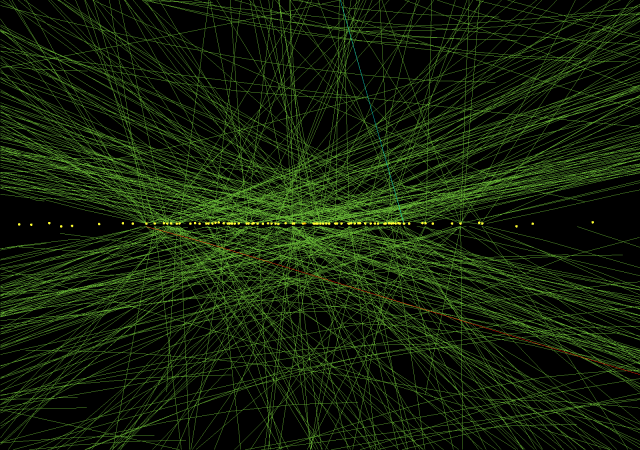
\includegraphics[width=0.6\textwidth]{tex/reco/fig/reco-vtx.png}
  \caption{An event display showing 78 vertices that were reconstructed using information from the CMS tracker.
    The yellow dots correspond to reconstructed vertices, and the green lines correspond to reconstructed
    tracks. The data used to make this figure was collected on July 10, 2012 using $pp$ collisions with a 
    center-of-mass energy of 8 TeV \cite{vtx-pictures}.}
  \label{fig:reco-vtx}
\end{figure}


Primary vertex reconstruction takes place once the prompt tracks in the event 
have been reconstructed.  Prompt tracks from the primary
interaction region are selected according to their impact parameter significance
($\text{IP}/\sigma_{\text{IP}}$) with respect to the beamspot, number of hits
in the pixel and silicon strip trackers, and normalized $\chi^2$ ($\chi^2/\text{ndof}$).
It is noteworthy that there is no requirement on track \pt, in order to 
ensure a high reconstruction efficiency.
Once these tracks have been selected, they are clustered according to the $z$ coordinate
at the point of their closest approach to the beamspot.
The clustering requires each track to have a separation in the $z$ coordinate ($z_{\text{sep}}$) of less than 1 cm
from its nearest neighbor.  Primary vertex candidates that have more than one track 
are fit with an adaptive vertex fit \cite{vtx-3}.
In this adaptive vertex fit, each track associated with a vertex is given a weight, $w$, between 0 and 1,
based on its compatibility with the vertex.  Tracks compatible with a given vertex have a
weight that is close to 1.  The variable ``number of degrees of freedom'' is defined as 
$n_{\text{dof}} = 2 \sum_{\text{tracks}}\left(w_i -3\right)$, where $w_i$ is the weight of the $i^{\text{th}}$ track.
Number of degrees of freedom is highly correlated with the number of tracks associated with a given vertex,
and this varible is used to identify real $pp$ interaction vertices \cite{vtx-2}.
An event display showing 78 reconstructed vertices in the $r-z$ plane is provided in Figure \ref{fig:reco-vtx}.
This display was made using data collected on July 10, 2012.

